\documentclass[../report.tex]{subfiles}
\begin{document}
\section{Phase 1 : Fonctionnalités de base}
Cette section documente le travail réalisé pour atteindre les fonctionnalités de base. On définit en tant que fonctionnalités de base le fait d'avoir un interpréteur capable de lire un fichier Prolog, et de répondre à des requêtes au clavier portant sur des faits simples.

Cette phase relativement simple nécessite déjà d'avoir toutes les technologies du projet fonctionnelles et travaillant ensemble.
\subsection{Besoins}
Les besoins de cette phase sont les suivants :
\begin{itemize}
    \item Préparation de l'environnement GraalVM et Truffle
    \item Lecture de fichiers
    \item Lexing et parsing de faits écrits en Prolog
    \item Récupération de l'entrée clavier et requêtes dans les faits lus
\end{itemize}
En plus de ces besoins technologiques, il faut également décider la "philosophie" et l'architecture générale de l'interpréteur.
\subsection{Approche}
Cette section décrit l'approche pour subvenir aux différents besoins.
\subsubsection{Choix d'une philosophie}
Afin de pouvoir choisir une architecture et une philosophie de développement pour l'interpréteur, une recherche préalable sur les implémentations existantes et sur les manières d'implémenter un interpréteur Prolog a été effectué. On apprend par exemple dans \cite{WarrenAM}(\citetitle{WarrenAM}) qu'il existe des techniques pour réaliser un interpréteur optimisé, mais ces techniques se reposent sur des mécanismes de bas niveau qui seraient difficiles à mettre en place avec Truffle, en tout cas dans un premier temps. 

Pour des exemples plus proches de ce que l'on cherche à réaliser, on trouve des implémentations en Java d'interpéteurs Prolog, par exemple \cite{JIProlog}(\citetitle{JIProlog}). Certaines de ces versions se basent sur une approche complètement orientée objet; c'est cette philosophie qui sera retenue pour notre implémentation.
\subsubsection{Technologies}
Pour prendre en main la technologie Truffle, quelques ressources sont à disposition en ligne. On trouve par exemple la conférence \cite{OneVM}\citetitle{OneVM} qui présente quelques aspects liés à Truffle. On trouve également une série d'articles de blog décrivant le parcours réalisé par un développeur californien pour implémenter son propre nouveau langage de programmation, d'abord en pur Java puis en intégrant Truffle (\cite{WritingTruffle}).

Mais la meilleur ressource disponible pour prendre en main la suite de technologies reste le projet de démonstration \citetitle{SimpleLanguage}, qui fournit un exemple complet et relativement bien documenté sur l'utilisation de toutes les technologies et des différents liens entre celles-ci.
\subsection{Plan}
Le plan de réalisation de cette phase est donc le suivant : prendre comme base l'implémentation de démonstration \sl, et commencer par retirer tout ce qui est spécifique à cette dernière, afin de se retrouver avec une base "minimale". Puis, les fonctionnalités propres à notre interpréteur seront rajoutées une à une à cette base, de manière incrémentale.
\subsection{Prise en main}\label{subsec:part1handling}
Le projet \sl{} se présente sous la forme d'un projet \textit{Maven}. Il est composé de quatre sous-parties : 
\begin{itemize}
    \item component : contient les fichiers nécessaires pour créer une version ajoutable à GraalVM (un \textit{plugin}).
    \item language : contient les sources de l'interpréteur du langage \sl{}
    \item launcher : contient les sources permettant de lancer l'interpréteur \sl{}
    \item native : contient les fichiers nécessaires pour créer une version "native" d'un programme \sl{}
\end{itemize}
Après l'installation de GraalVM et de Maven, puis la mise en place des variables d'enviromments nécessaires (opérations décrites en annexe de ce document), on peut taper \mintinline{bash}{mvn package} pour créer les différents fichiers JAR correspondant aux parties du projet \sl{}. On peut ensuite utiliser le script fourni, sobrement appelé "sl", pour lancer l'interpréteur fraîchement compilé en lui donnant un des fichiers ".sl" fourni et vérifier que tout fonctionne.
\subsection{Implémentation}
Maintenant que l'on sait que tout compile et fonctionne, on peut commencer à retirer les fonctionnalités propres à \sl{} pour obtenir notre base pour la suite. On commence donc par supprimer les sous-parties "component" et "native" qui ne seront pas utilisées pour l'instant. On continue en modifiant les différents fichiers de description de projet Maven "pom.xml" afin de modifier le nom du projet en "ProloGraal", nom original pour le sous-ensemble de fonctionnalités Prolog développé lors de ce projet. On peut ensuite commencer à étudier le code fourni, en commençant par le launcher, vu que celui-ci est composé uniquement d'une seule classe.
\subsection{Implémentation : launcher}
Le launcher contient le "main" de l'application, et permet donc de lancer l'interpréteur de manière autonome. Il se charge de créer une représentation abstraite du code source à exécuter à l'aide d'un objet de type \mintinline{Java}{Source} et est également responsable de la création d'un contexte d'exécution pour ce code source, en lui donnant notamment les flux d'entrée et de sortie. Ce mécanisme est pratique car il permet de donner des flux fictifs pour les tests unitaires par exemple (cf. section \ref{sec:unittests}).

Au final on se rend compte que tout le code déjà existant est assez générique, et qu'il suffit de remplacer les références au langage SL par des références vers le nôtre.
\begin{minted}{Java}
private static final String SL = "sl";
// devient
private static final String PROLOGRAAL = "pl";
\end{minted}
\subsection{Implémentation : language}
Le launcher étant terminé pour le moment, on peut passer au gros morceau : le composant language. Ce composant contient tout le code propre à \sl{}, du lexer au parser en passant par le code Truffle. Il va donc falloir trier les fonctionnalités afin de distinguer celles qui nous seront utiles telles quelles, celles qui devront être adapatées et celles qui peuvent être supprimées.

On commence en étudiant la structure du code. La figure \ref{fig:simplelanguagestructure} donne un aperçu de celle-ci.
\begin{figure}[h]
    \centering
    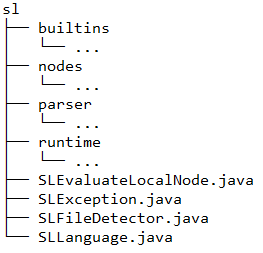
\includegraphics[]{simplelanguagestructure.png}
    \caption{Structure du code du module "language" de \sl{}}
    \label{fig:simplelanguagestructure}
\end{figure}
On distingue quatre packages et quelques fichiers racines. Ces packages sont les suivants :
\begin{itemize}
    \item builtins : contient des classes décrivant des méthodes prédéfinies propres au langage SL. A priori ne semble pas intéressant, vu que le contenu est très spécifique.
    \item nodes : contient des classes décrivant des bouts de code (\textit{statements}) SL. Bien que le code soit à nouveau spécifique, la structure est néanmoins intéressante pour la suite.
    \item parser : contient les classes gérant le lexing et le parsing d'un fichier source SL. Contient également un fichier ".g4" qui est un fichier de grammaire ANTLR servant à décrire le langage SL. Ce package est donc intéressant pour ce que l'on souhaite réaliser à ce stade.
    \item runtime :  contient des classes décrivant les types propres à SL ainsi qu'un conteneur de contexte \mintinline{text}{SLContext.java}. Comme pour le package "nodes", la structure est intéressante, particulièrement le conteneur de contexte qui se retrouvera sûrement dans notre interpréteur.
\end{itemize}
Parmi les fichiers racines, les fichiers intéressants semblent être \mintinline{text}{SLFileDetector.java}, qui permet de vérifier qu'un fichier contient du code SL, et \mintinline{text}{SLLanguage.java} qui semble être le fichier principal du module.
\subsubsection{Point d'entrée : Analyse}
\label{subsubsec:entrypoint}
On va maintenant repartir du fichier principal trouvé précédemment, \mintinline{text}{SLLanguage.java}, et analyser son contenu. Il contient une classe \mintinline{text}{SLLanguage} héritant de \mintinline{text}{TruffleLanguage<SLContext>}. Cette classe est précédée d'une annotation décrivant le nom de langage et lui donnant un ID. Elle redéfinit plusieurs méthodes, et certaines semblent particulièrement intéressantes : \mintinline{text}{createContext} et \mintinline{text}{parse}.

On commence par la fonction \mintinline{text}{parse}. On comprend qu'elle utilise le parser pour récupérer la liste des fonctions présentes dans le fichier sous la forme d'une \mintinline{Java}{Map<String, RootCallTarget>}. Les \mintinline{Java}{RootCallTarget} sont des objets de Truffle représentant des racines de l'arbre de syntaxe abstrait, autrement dit, ils représentent des fonctions appelables. Une fois la liste des fonctions récupérée, la méthode récupère la fonction "main" si elle existe et crée un noeud de type \mintinline{Java}{SLEvalRootNode} en lui donnant cette fonction. Finalement la méthode retourne un \mintinline{Java}{CallTarget} contenant cet \mintinline{Java}{SLEvalRootNode} via l'environnement Truffle :\\
\mintinline{Java}{Truffle.getRuntime().createCallTarget(evalMain)}

Un \mintinline{Java}{CallTarget} représente du code appelable. Ici, le \mintinline{Java}{CallTarget} sera invoqué automatiquement plus tard par Truffle.
\subsubsection{Point d'entrée : Modifications}
Pour guider nos modifications, on peut assimiler la liste de fonctions à la liste des faits du programme Prolog. On doit donc modifier le parser, premièrement pour qu'il fonctionne pour du Prolog et plus du SL, mais également pour qu'il retourne correctement la liste de faits. Il faut également adapter le \mintinline{Java}{SLEvalRootNode}.

Concernant les autres méthodes de la classe, leur utilité restant pour le moment floue, elles sont réduites au minimum et laissées de côté.
\subsubsection{Parser : Analyse}
Le parser se compose de quatre parties principales :
\begin{itemize}
    \item \mintinline{text}{SimpleLanguage.g4} qui est le fichier de grammaire ANTLR décrivant comment lexer et parser un fichier SL. ANTLR s'en sert pour générer le lexer et le parser en Java. Il contient également des bouts de code permettant d'invoquer des appels à la \mintinline{Java}{SLNodeFactory} décrite plus bas.
    \item \mintinline{text}{SimpleLanguageLexer.java} qui est un fichier généré automatiquement par ANTLR et qui contient le code Java nécessaire au lexing d'un fichier SL.
    \item \mintinline{text}{SimpleLanguageParser.java} qui est un fichier généré automatiquement par ANTLR et qui contient le code Java nécessaire au parsing d'un fichier SL.
    \item \mintinline{text}{SLNodeFactory.java} qui contient le code appelé depuis celui généré par ANTLR. Il s'agit d'une "Factory", ou usine, qui est un patron de développement faciliant la création d'objets. En l'occurrence, cette Factory permet de créer les différents noeuds Truffle représentant les parties du code source SL.
\end{itemize}
La grammaire et la Factory vont donc devoir être modifiées pour fonctionner avec du Prolog. Mais avant, il faut décider comment on va représenter du code Prolog de manière abstraite à l'aide de classes.
\subsection{Représentation des éléments}
\label{subsec:prologRules}
Pour représenter un code Prolog en Java, un rappel sur Prolog s'impose. On sait des standards (\cite{PrologSyntax}) que Prolog contient une seule unité de données, le terme. Un terme peut être de plusieurs types :
\begin{itemize}
    \item un atome : un atome est une séquence de caractères, qui ne transporte pas d'informations supplémentaires
    \item un nombre : les nombres en Prolog peuvent être de type entier ou à virgule flottante
    \item une variable : les variables en Prolog ont la fonction des variables en logique; elles peuvent être remplacées par un autre type de données pour satisfaire une requête
    \item un terme composé : un terme composé est constitué d'un atome appelé foncteur et d'un certain nombre d'arguments. Ces arguments sont eux-mêmes des termes. Le nombre d'arguments d'un terme composé est appelé arité.
\end{itemize}
Il est maintenant trivial de transposer cette hiérarchie en Java. La figure \ref{fig:part1classdiagram} montre une représentation possible de ces différents types, en omettant volontairement les variables car nous ne nous en occuperons pas encore dans cette phase.
\begin{figure}[h]
    \centering
    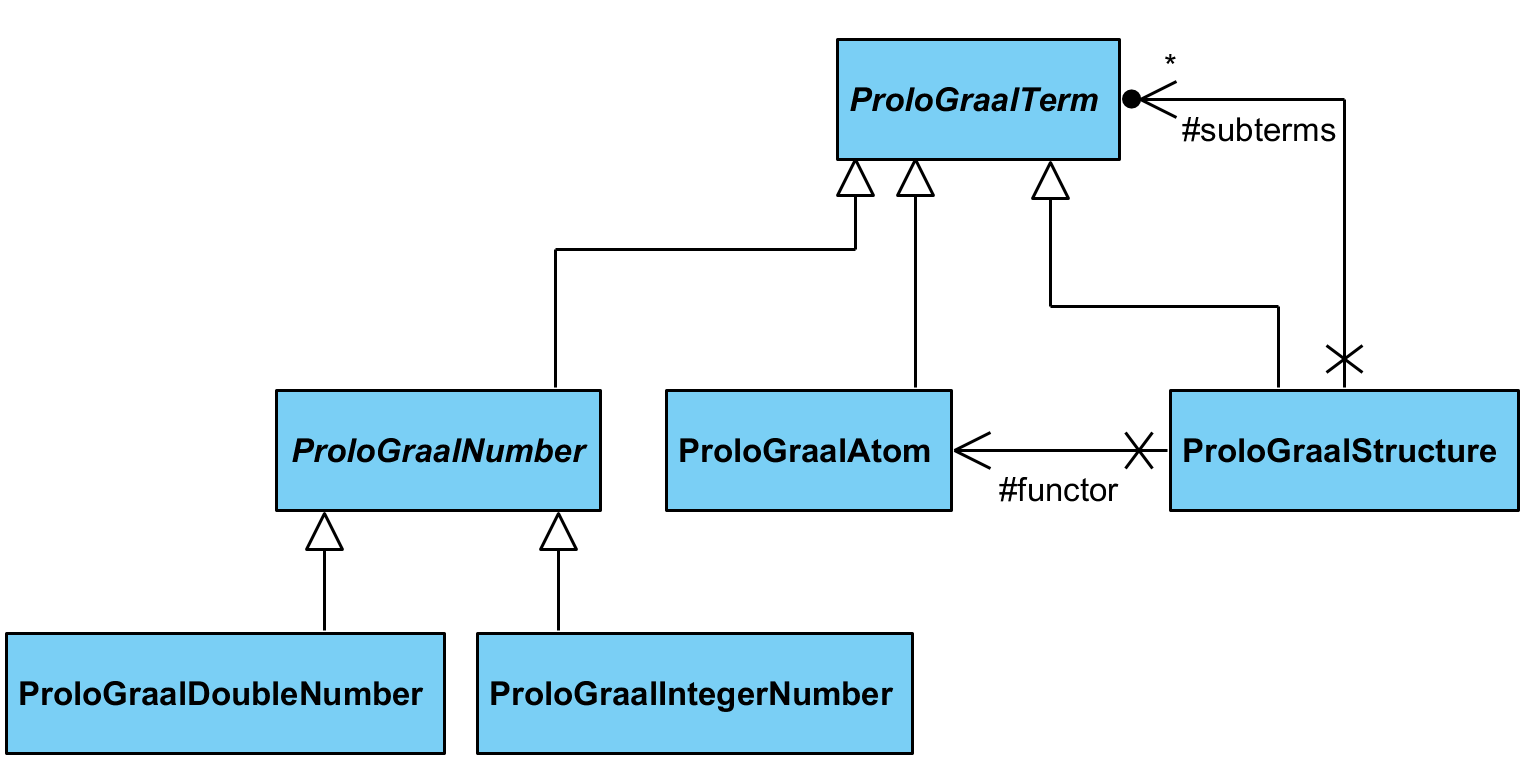
\includegraphics[width=\textwidth]{part1classdiagram.png}
    \caption{Diagramme de classes des éléments Prolog en Java}
    \label{fig:part1classdiagram}
\end{figure}

En plus des données, un concept vital à Prolog est la réussite ou l'échec d'une requête. On pourrait représenter cela à l'aide d'un simple booléen en Java, mais le choix d'abstraire cette représentation à l'aide de nouvelles classes a été fait, en prévision pour les phases suivantes. La figure \ref{fig:part1classdiagram2} montre la représentation choisie pour ce concept.
\begin{figure}[h]
    \centering
    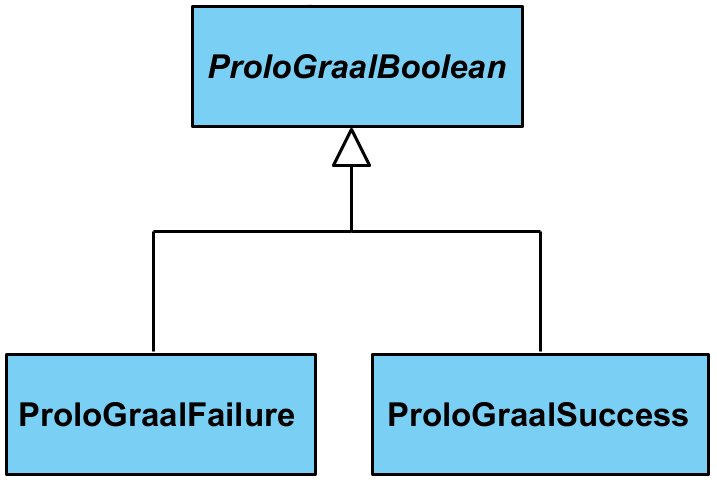
\includegraphics[width=0.5\textwidth]{part1classdiagram2.png}
    \caption{Diagramme de classes représentant la réussite et l'échec Prolog en Java}
    \label{fig:part1classdiagram2}
\end{figure}
\subsection{Implémentation : parser}
Maintenant que nous avons la structure des éléments représentée en Java, il faut écrire une grammaire ANTLR permettant de générer le code. Pour démarrer l'implémentation, nous avons les pistes suivantes : la grammaire de \sl{}, et l'excellent tutoriel \cite{ANTLRTutorial}. Après lecture de ce tutoriel, il est possible d'analyser la grammaire écrite pour \sl{}. On se rend compte qu'elle utilise une méthode hybride, avec du code Java imbriqué dans la grammaire, pour faire des appels à une autre classe se chargeant de créer les représentations Java des différents éléments au fur et à mesure. Cette méthode n'est pas particulièrement lisible, et elle n'est également pas recommandée par ANTLR. Les méthodes recommandées par ANTLR suivent deux patterns de développement :
\begin{itemize}
    \item Le pattern Visitor
    \item Le pattern Listener
\end{itemize}
Le pattern Visitor est un peu plus flexible mais plus compliqué à mettre en place que le pattern Listener. Le langage Prolog n'étant pas particulièrement difficile à parser et à transformer en Java, le pattern Listener a donc été retenu pour sa simplicité d'implémentation.

Ces choix techniques effectués, il reste le principal : écrire la grammaire. ANTLR sépare les règles de lexing et les règles de parsing.
\subsubsection{Lexer}
Comme décrit précédemment, Prolog ne contient pas beaucoup de symboles différents. Pour cette première phase, on en distingue uniquement deux : les atomes et les nombres.

Un atome commence par une lettre minuscule, et peut être suivi d'un certain nombre de caractères, pouvant être des lettres minuscules ou majuscules, des chiffres, ou un underscore. Un atome peut également commencer par une apostrophe et contenir n'importe quel caractère jusqu'à rencontrer une nouvelle apostrophe. Voici comment se traduisent ces règles dans une grammaire ANTLR :
\begin{minted}{ANTLR}
ATOM : (LOWERCASE+ (LOWERCASE | UPPERCASE | DIGITS | '_')*) | ('\'' .*? '\'');
\end{minted}
Pour rendre la règle plus lisible, des fragments sont utilisés. Les fragments sont des sortes de macro remplaçant une certaine classe de caractères :
\begin{minted}{ANTLR}
fragment LOWERCASE : [a-z];
fragment UPPERCASE : [A-Z];
fragment DIGITS : [0-9];    
\end{minted}
Pour les nombres, ceux-ci doivent commencer par un chiffre, et être suivis d'un certain nombre d'autres chiffres. Ils peuvent également contenir un point suivi d'autres chiffres encore pour repésenter un nombre à virgule. D'autres notations sont disponibles en Prolog classique, comme la notation exponentielle par exemple, mais pour des raisons de simplicité, celles-ci sont omises. Voici l'implémentation de ces règles :
\begin{minted}{ANTLR}
NUMBER : DIGITS+ ('.' DIGITS+)?;
\end{minted}
Nous devons encore définir des règles pour les espaces blancs et les commentaires, tous deux devant être ignorés :
\begin{minted}{ANTLR}
WHITESPACE : [ \t\r\n]+ -> skip;
COMMENT : '%' ~[\r\n]* -> skip;    
\end{minted}
On définit encore un dernier élément de lexing, le caractère terminal point servant à délimiter les différentes clauses du programmes :
\begin{minted}{ANTLR}
TERMINATOR : '.';
\end{minted}
La partie lexer est maintenant terminée pour cette phase, on peut maintenant utiliser ces règles pour écrire les règles de parsing.
\subsubsection{Parser}
Pour la partie parser, on se base sur les règles définies à la section \ref{subsec:prologRules}. On sait également qu'un programme Prolog est composé d'un certain nombre de clauses. Pour cette phase, nous savons que ces clauses seront uniquement des faits. Ces règles se traduisent à nouveau de manière très élégante dans la grammaire ANTLR :
\begin{minted}{ANTLR}
prolograal
:
clause clause* EOF
;

clause
:
fact
;

fact
:
term TERMINATOR
;
\end{minted}
Comme décrit à la section \ref{subsec:prologRules}, un terme peut être de plusieurs types. On retrouve ces différentes possibilités dans la grammaire :
\begin{minted}{ANTLR}
term
:
functor 
(
    '(' term (',' term)* ')'
) |
atom | 
number
;    
\end{minted}
Le reste des éléments ne sera pas détaillé, mais il s'agit à chaque fois d'une chaîne de règles se terminant par un élément dit "terminal", qui contient uniquement une référence vers un élément du lexer. Par exemple pour un atome :
\begin{minted}{ANTLR}
atom
:
ATOM
;    
\end{minted}
La grammaire est ensuite testée en utilisant un outil fourni par ANTLR permettant de visualiser l'arbre de syntaxe généré après le parcours d'un fichier. La figure \ref{fig:antlr1} montre et valide le résultat obtenu avec la grammaire actuelle, pour le fichier d'exemple Prolog suivant :
\begin{minted}{Prolog}
hello(world).
test(antlr).
multiples(arg1, arg2).
\end{minted}
\begin{figure}[h]
    \centering
    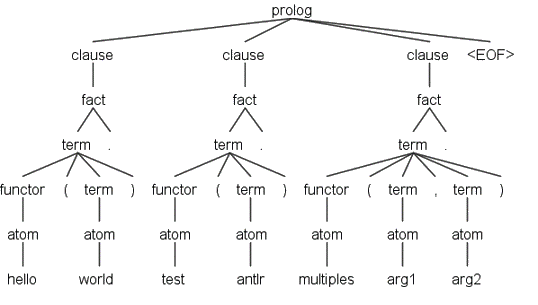
\includegraphics{ANTLR1.png}
    \caption{Arbre de syntaxe obtenu après le parcours d'un fichier Prolog en utilisant la grammaire ANTLR de la phase 1}
    \label{fig:antlr1}
\end{figure}
\subsubsection{Génération des fichiers Java}
Pour générer les fichiers Java correspondant à la grammaire, on utilise l'exécutable JAR de ANTLR. Des explications détaillées sur l'utilisation de ce JAR sont disponibles dans le guide d'installation fourni en annexe (Annexe \ref{subsec:manual}). Cet exécutable génère plusieurs fichiers :
\begin{itemize}
    \item ProloGraalLexer.java : fichier contenant le code du lexer
    \item ProloGraalParser.java : fichier contenant le code du parser
    \item ProloGraalListener.java : interface Java décrivant les fonctions à implémenter pour le pattern Listener. L'interface définit deux méthodes pour chaque élément du parser : une méthode "enter" et une méthode "exit". Ces méthodes seront appelées automatiquement lorque l'on parcourra le fichier. 
    \item ProloGraalBaseListener.java : implémentation vide de l'interface Java du Listener
\end{itemize}
L'étape suivante est donc de créer une classe héritant de l'implémentation vide du Listener, pour ajouter la logique permettant de créer nos éléments Java correctement pendant le parcours du fichier source Prolog.
\subsubsection{Implémentation du listener}
\label{subsubsec:listenerImpl}
L'implémentation du listener de parcours se base sur le principe suivant : on doit obtenir au final la liste des différents termes qui sont à la racine du fichier (qui sont donc les différents faits). La principale difficulté à surmonter est le fait que les termes composés peuvent être imbriqués. Par exemple, quand on entre dans un atome dans le listener, il est impossible de savoir si l'on est dans une structure imbriquée, et si oui dans laquelle on se trouve. En raison de cela, pour suivre le contexte actuel, les structures de données suivantes sont utilisées :
\begin{itemize}
    \item une liste de termes pour stocker les termes racines
    \item une pile d'atomes représentant les foncteurs. Le sommet de la pile représente donc le foncteur de la structure la plus récente.
    \item une pile de listes de termes, représentant les arguments de chaque structure. Le sommet de la pile représente donc les arguments de la structure la plus récente.
\end{itemize}
En plus de ces structures, un compteur de profondeur sera également tenu à jour, incrémenté lors de l'entrée dans un terme possédant plus d'un descendant (terme composé), et décrémenté à la sortie de ceux-ci. Ce compteur est nécessaire pour choisir s'il faut ajouter le terme courant à la liste des arguments de la structure courante, ou directement à la liste des faits (si la profondeur est égale à 0).\footnote{en rétrospective, ce compteur n'est pas utile et aurait pu être remplacé par une simple vérification de la taille de la pile de foncteurs (si elle est vide, nous sommes à la racine...)}

On commence donc par initialiser nos différentes structures au moment de l'entrée dans le fichier :
\begin{minted}{Java}
public void enterProlograal(ProloGraalParser.ProlograalContext ctx) {
    clauses = new ArrayList<>();
    structArgs = new Stack<>();
    functors = new Stack<>();
    depth = 0;
}
\end{minted}
Lorsque l'on entre dans un terme, si celui-ci a plus d'un enfant, alors il s'agit d'un terme composé, et il faut donc incrémenter le compteur de profondeur en conséquence :
\begin{minted}{Java}
public void enterTerm(ProloGraalParser.TermContext ctx) {
    if (ctx.getChildCount() > 1)
        depth++;
}
\end{minted}
Lorsque l'on sort d'un terme, si celui-ci a plus d'un enfant, alors il faut décrémenter le compteur de profondeur, créer un nouveau terme composé avec le foncteur et les arguments les plus récents (ceux au sommet des piles), et ajouter cette nouvelle structure :
\begin{minted}[breaklines]{Java}
public void exitTerm(ProloGraalParser.TermContext ctx) {
    if (ctx.getChildCount() > 1) {
        depth--;
        ProloGraalStructure struct = new ProloGraalStructure(functors.pop(), structArgs.pop());
        add(struct);
    }
}
\end{minted}
Lorsque l'on ajoute un élément, il faut l'ajouter au bon endroit. Si la profondeur est à zéro, cela signifie que nous sommes à la racine, et il faut donc ajouter l'élément directement à la liste des faits. Sinon, il faut l'ajouter à la liste des arguments du terme composé le plus récent :
\begin{minted}{Java}
private void add(ProloGraalTerm term) {
    if (depth == 0)
        clauses.add(term);
    else
        structArgs.peek().add(term);
}
\end{minted}
Lorsque l'on entre dans un atome, il faut vérifier s'il s'agit d'un foncteur ou non. S'il s'agit d'un foncteur, la logique est gérée au moment de l'entrée dans un foncteur et il ne faut donc rien faire de plus. Sinon, il faut simplement créer un nouvel atome et l'ajouter :
\begin{minted}{Java}
public void enterAtom(ProloGraalParser.AtomContext ctx) {
    // if the parent is a functor
    if (ctx.parent instanceof ProloGraalParser.FunctorContext) {
        return; // already handled
    }
    add(new ProloGraalAtom(ctx.getText()));
}
\end{minted}
Lorsque l'on entre dans un foncteur, il faut créer un nouvel atome pour ce foncteur et l'ajouter à la pile des foncteurs. Il faut également créer une nouvelle liste d'arguments et l'ajouter à sa pile :
\begin{minted}{Java}
public void enterFunctor(ProloGraalParser.FunctorContext ctx) {
    functors.push(new ProloGraalAtom(ctx.getText()));
    structArgs.push(new ArrayList<>());
}
\end{minted}
Restent uniquement les nombres, qui doivent juste être créés avec le bon type, entier ou à virgule, puis ajoutés :
\begin{minted}{Java}
public void enterNumber(ProloGraalParser.NumberContext ctx) {
    String n = ctx.getText();
    try {
        add(new ProloGraalIntegerNumber(Integer.parseInt(n)));
    } catch (NumberFormatException ex) {
        add(new ProloGraalDoubleNumber(Double.parseDouble(n)));
    }
}
\end{minted}
\subsection{Implémentation : language (suite)}
La partie parser étant terminée, il est temps de la lier avec la partie principale. Faisons d'abord un point sur ce que nous avons actuellement :
\begin{itemize}
    \item un parser fonctionnel, nous retournant la liste des faits du programmes sous la forme de termes (section \ref{subsubsec:listenerImpl})
    \item une représentation en Java de ces termes (section \ref{subsec:prologRules} et figure \ref{fig:part1classdiagram})
    \item une représentation en Java des concepts de succès et d'échec (section \ref{subsec:prologRules} et figure \ref{fig:part1classdiagram2})
    \item une compréhension basique du fonctionnement de la partie principale (section \ref{subsubsec:entrypoint})
\end{itemize}
On va donc maintenant repartir de cette partie principale, et la lier à notre parser en récupérant la liste des différents faits. 
\subsubsection{Liaison au parser}
Dans \sl{}, l'appel au parser se fait via une méthode statique rajoutée dans le parser généré par ANTLR, appelée \mintinline{Java}{parseSL}. On va donc simplement copier cette méthode et l'adapter à notre fonctionnement dans une nouvelle classe.

Cette méthode est relativement triviale. Elle crée une instance du lexer et du parser, et donne au lexer le fichier source qu'elle reçoit en paramètre. Elle attache également un écouteur d'erreur à ces deux instances. Enfin, elle récupère un \mintinline{Java}{ParseTree} depuis le parser, représentant l'arbre de syntaxe du fichier. On peut donc facilement l'adapter pour qu'elle utilise notre lexer et parser :
\begin{minted}[breaklines]{Java}
public static List<ProloGraalTerm> parseProloGraal(ProloGraalLanguage language, Source source) {
    ProloGraalLexer lexer = new ProloGraalLexer(CharStreams.fromString(source.getCharacters().toString()));
    ProloGraalParser parser = new ProloGraalParser(new CommonTokenStream(lexer));
    lexer.removeErrorListeners();
    parser.removeErrorListeners();
    BailoutErrorListener errListener = new BailoutErrorListener(source);
    lexer.addErrorListener(errListener);
    parser.addErrorListener(errListener);
    ProloGraalParserImpl.source = source;
    ParseTree tree = parser.prolograal();
    // ...
\end{minted}
Il reste à ajouter le code nécessaire pour utiliser notre listener. Il faut en créer une instance, et l'appeler à l'aide d'un \mintinline{Java}{ParseTreeWalker}. Le \mintinline{Java}{ParseTreeWalker} se charge d'appeler les méthodes "enter" et "exit" au bon moment. Enfin, il faut également retourner la liste des faits à l'appelant :
\begin{minted}[breaklines]{Java}
    // ...
    ProloGraalListenerImpl listener = new ProloGraalListenerImpl();
    ParseTreeWalker.DEFAULT.walk(listener, tree);

    listener.debug();

    return listener.getClauses();
}
\end{minted}
On peut maintenant récupérer les clauses dans notre fichier principal :
\begin{minted}{Java}
clauses = ProloGraalParserImpl.parseProloGraal(this, source);
\end{minted}
\subsubsection{Interpréteur : Analyse}
Nous pouvons maintenant lire un fichier Prolog, et manipuler les faits qu'il contient en Java. Il nous faut donc à présent en faire quelque chose. Pour cela, nous avons besoin d'un interpréteur pour lire les requêtes de l'utilisateur.

Deux endroits sont possibles pour l'implémentation d'un tel interpréteur :
\begin{itemize}
    \item Dans la partie "launcher". L'interpréteur serait externe au langage même, et il faudrait trouver un mécanisme pour envoyer les requêtes et récupérer leurs résultats.
    \item Directement dans la partie "language". L'interpréteur serait donc interne et fortement lié au langage, ce qui facilite le traitement des requêtes.
\end{itemize}
Le second choix semble donc meilleur. De plus, \sl{} possède une implémentation des fonctions "eval" (permettant d'évaluer du code à la volée) et "read" (permettant de lire l'entrée standard), qui sont précisément ce que l'on va chercher à faire. Conceptuellement, nous allons donc faire comme si notre fichier Prolog se terminait toujours par une instruction "read" qui enverrait son contenu à une fonction "eval".

Mais d'abord, il faut encore se pencher sur le \mintinline{Java}{EvalRootNode} qui est, comme indiqué à la section \ref{subsubsec:entrypoint}, le point d'entrée du programme après le parsing du code source.
\subsubsection{Adaptation du \texttt{EvalRootNode} : analyse}
Dans la classe \mintinline{Java}{SLEvalRootNode}, on trouve une méthode particulièrement intéressante : la méthode \mintinline{Java}{execute}. Cette méthode sauvegarde les fonctions obtenues après l'évaluation du code source dans le contexte, et crée un nouveau noeud pour la fonction "main", qui est ensuite appelé. Dans notre cas, les fonctions correspondent aux prédicats Prolog, et il n'existe pas de prédicat "main". On en déduit donc deux modifications à effectuer : adapter le contexte pour qu'il puisse sauvegarder nos faits, et créer puis exécuter un noeud pour notre interpréteur, qui sera l'équivalent de notre fonction "main".
\subsubsection{Adaptation du contexte}
Le contexte de \sl{}, \mintinline{Java}{SLContext}, contient de nombreuses méthodes. Celles qui nous intéressent actuellement sont : les méthodes pour récupérer les flux d'entrée et de sortie, qui nous seront utiles pour l'interpréteur, et la méthode pour récupérer le \mintinline{Java}{SLFunctionRegistry}. On va donc simplifier la classe : on enlève toutes les méthodes qui n'ont pas l'air utile pour le moment. On garde les méthodes d'entrée/sortie, sans même avoir besoin de les adapter. On enlève également le \mintinline{Java}{SLFunctionRegistry}, que l'on remplace par une simple liste de termes correspondant à nos faits. Nous obtenons un contexte capable de stocker nos faits et de fournir les flux d'entrée et de sortie, tout ce dont nous avons besoin pour réaliser l'interpréteur.
\subsubsection{Adaptation du \texttt{EvalRootNode} : implémentation}
Le contexte étant maintenant prêt, on peut adapter le \mintinline{Java}{EvalRootNode}. On enregistre les clauses dans le contexte :
\begin{minted}{Java}
reference.get().registerClauses(clauses);
\end{minted}
On va également créer et enregister dans le contexte les noeuds d'interprétation et de résolution (discutés dans les sections suivantes), puis finalement invoquer le noeud d'interprétation.
\begin{minted}[breaklines]{Java}
ProloGraalInterpreterNode interpreterNode = new ProloGraalInterpreterNode(language);
ProloGraalResolverNode resolverNode = new ProloGraalResolverNode(language);

reference.get().registerInterpreter(interpreterNode);
reference.get().registerResolver(resolverNode);
// ...

return Truffle.getRuntime()
    .createCallTarget(reference.get().getInterpreterNode()).call();
\end{minted}

\subsubsection{Interpréteur : Implémentation}
En s'inspirant du code des fonctions d'évaluation et de lecture d'entrée de \sl{}, \mintinline{Java}{SLEvalBuiltin} et \mintinline{Java}{SLReadInBuiltin}, on crée une classe \mintinline{Java}{ProloGraalInterpreterNode} qui hérite de \mintinline{Java}{RootNode}, ce qui lui permet d'être exécutée via sa méthode \mintinline{Java}{execute}. Le déroulement de cette méthode est très simple : on lit l'entrée standard, on parse la ligne ainsi obtenue, on exécute cette ligne et on affiche le succès ou l'échec de l'opération, puis on recommence toutes ces opérations jusqu'à l'arrêt du programme par l'utilisateur.

Pour interpréter la ligne lue, on peut réutiliser le parser principal, de la même façon que pour lire le fichier Prolog initial :
\begin{minted}[breaklines]{Java}
Source source = Source.newBuilder("pl", line, null).build();
List<ProloGraalTerm> terms = ProloGraalParserImpl.parseProloGraal(language, source);
\end{minted}
Il faut ensuite vérifier que l'on a bien lu un fait, et surtout lancer le processus pour vérifier si ce fait est présent dans ceux lus depuis le fichier Prolog. Cette tâche étant vouée à devenir de plus en plus complexe au fil du projet, il a été décidé de séparer le traitement dans une nouvelle classe, le \mintinline{Java}{ProloGraalResolverNode}. Comme pour l'interpréteur, cette classe sera de type \mintinline{Java}{RootNode}. On lui fournit la liste des clauses lues depuis l'entrée standard (pour l'instant, il doit y en avoir exactement une), et elle doit nous retourner si oui ou non la clause est compatible avec un des faits de la liste construite depuis le fichier Prolog.

Dans l'interpréteur, ces opérations prennent la forme suivante :
\begin{minted}[breaklines]{Java}
System.out.println(Truffle.getRuntime()
    .createCallTarget(context.getResolverNode()).call(terms));
\end{minted}
\subsubsection{Noeud de résolution}
Pour cette phase, il n'y pas de variables ou de clauses, uniquement des faits, et on ne gère que le cas où la requête est composée d'un unique fait. Le noeud de résolution doit donc uniquement trouver un fait dans la liste construite depuis le fichier Prolog qui est exactement égal au fait que l'on reçoit depuis l'interpréteur. Comme pour l'interpréteur, ce noeud hérite de \mintinline{Java}{RootNode} et a donc une méthode \mintinline{Java}{execute} qui sera appelée par Truffle.

Récupération du but, qui est le fait dont on veut vérifier l'existence :
\begin{minted}{Java}
ProloGraalTerm goal = ((List<ProloGraalTerm>) frame.getArguments()[0]).get(0);
\end{minted}
Vérification de l'existence du fait dans la liste :
\begin{minted}{Java}
return ProloGraalBoolean
    .fromBoolean(terms.stream().anyMatch(x -> x.equals(goal)));
\end{minted}
Cette implémentation se base sur la méthode "equals", ce qui implique que tous nos termes implémentent correctement cette méthode. On s'en asssure en déclarant cette méthode comme abstraite dans notre classe de base, \mintinline{Java}{ProloGraalTerm} (cf. section \ref{subsec:prologRules}, figure \ref{fig:part1classdiagram}):
\begin{minted}{Java}
@Override
public abstract boolean equals(Object obj);
\end{minted}
À ce stade, vu qu'il n'y pas de variables, l'implémentation est triviale pour les atomes et les nombres, où il faut simplement vérifier qu'ils ont le même nom/la même valeur. Pour les structures, on doit vérifier récursivement chaque sous-terme :
\begin{minted}{Java}
if(obj == null) return false;
if(!(obj instanceof ProloGraalStructure)) return false;
ProloGraalStructure other = (ProloGraalStructure)obj;
return subterms.equals(other.subterms);
\end{minted}
Ceci conclut l'implémentation du noeud de résolution, et de la phase 1 du projet.
\subsection{Synthèse}
La phase 1 du projet est maintenant terminée. Voici ce que nous avons actuellement :
\begin{itemize}
    \item Un parser capable de transformer un fichier Prolog en sa représentation Java. Ce parser est pour l'instant capable de comprendre des faits, composés d'atomes, de nombres et de structures composées, mais pas de variables. Il est également réutilisable pour transformer l'entrée standard en sa représentation Java dans l'interpréteur.
    \item Une représentation "intelligente" des différents types de termes Prolog, capable de vérifier si un terme est exactement égal à un autre.
    \item Un contexte stockant la liste des faits obtenus depuis le parser, ainsi que les références vers l'interpréteur et le noeud de résolution.
    \item Un interpréteur capable de lire l'entrée standard, d'interpréter une ligne reçue depuis cette entrée à l'aide du parser et de demander au noeud de résolution de vérifier si cette ligne produit un succès ou un échec.
    \item Un noeud de résolution très simple capable de vérifier via l'intelligence des types si le fait reçu est exactement égal à un des faits présents dans la liste du contexte.
\end{itemize}
\end{document}